\newpage
\section{Kết quả và giải thích}
Do đã cài đặt alias cho các lệnh biên dịch nên việc biên dịch và chạy chương trình rất thuận tiện, chỉ với 1 câu lệnh \textbf{arm64 <tên\_file>}. Dưới đây là đoạn script chứa các lệnh biên dịch và chạy chương trình cho các bài tập:
\begin{figure}[H]
	\centering
	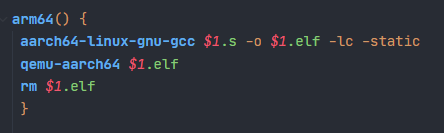
\includegraphics[width=\textwidth]{images/img0.PNG}
	\caption{Script biên dịch và chạy chương trình.}
\end{figure}
\subsection{Bài 1}
Viết chương trình nhập số nguyên n. Kiểm tra n có là số nguyên tố hay không?


\begin{figure}[H]
	\centering
	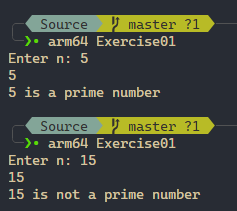
\includegraphics[width=10cm]{images/img1.PNG}
	\caption{Chụp màn hình kết quả bài 1 với 5 là số nguyên tố và 15 không phải là số nguyên tố.}
\end{figure}

\subsection{Bài 2}

Viết chương trình nhập số nguyên n. Kiểm tra n có là số nguyên hoàn thiện hay không?

\begin{figure}[H]
	\centering
	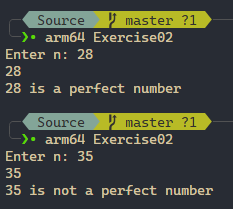
\includegraphics[width=10cm]{images/img2.PNG}
	\caption{Chụp màn hình kết quả bài 2 với 28 là số hoàn thiện và 35 không là số hoàn thiện.}
\end{figure}

\subsection{Bài 3}

Viết chương trình nhập vào số nguyên n. Kiểm tra n có là số chính phương hay không?

\begin{figure}[H]
	\centering
	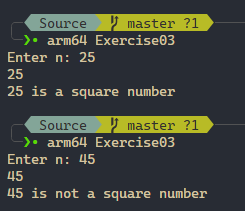
\includegraphics[width=10cm]{images/img3.PNG}
	\caption{Chụp màn hình kết quả bài 3 với 25 là số chính phương và 45 không là số chính phương.}
\end{figure}

\subsection{Bài 4}

Viết chương trình nhập số nguyên n. Kiểm tra n có là số đối xưng hay không?

\begin{figure}[H]
	\centering
	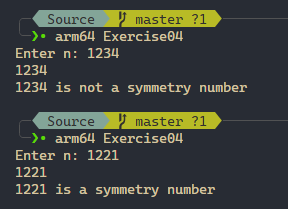
\includegraphics[width=10cm]{images/img4.PNG}
	\caption{Chụp màn hình kết quả bài 4 với 1221 là số đối xứng và 1234 không là số đối xứng.}
\end{figure}

\subsection{Bài 5}

Viết chương trình thực hiện các chức năng sau:
\begin{itemize}
	\item Nhập mảng 1 chiều n phần tử số nguyên.
	\item Xuất mảng
	\item Liệt kê các số nguyên tố
	\item Tìm giá trị lớn nhất trong mảng
	\item Tính trung bình mảng
\end{itemize}

\begin{figure}[H]
	\centering
	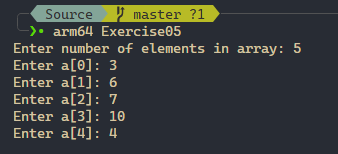
\includegraphics[width=10cm]{images/img5_0.PNG}
	\caption{Chụp màn hình chức năng nhập mảng với thứ tự nhập là 3, 6, 7, 10, 4}
\end{figure}

\begin{figure}[H]
	\centering
	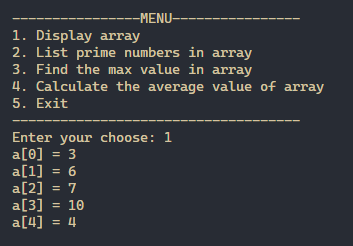
\includegraphics[width=10cm]{images/img5_1.PNG}
	\caption{Chụp màn hình chức năng xuất mảng với dữ liệu mảng đầu vào như trên.}
\end{figure}

\begin{figure}[H]
	\centering
	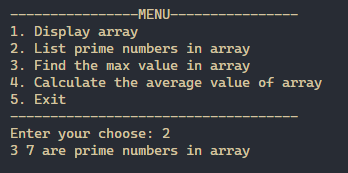
\includegraphics[width=10cm]{images/img5_2.PNG}
	\caption{Chụp màn hình chức năng liệt kê số nguyên tố với dữ liệu mảng đầu vào như trên.}
\end{figure}

\begin{figure}[H]
	\centering
	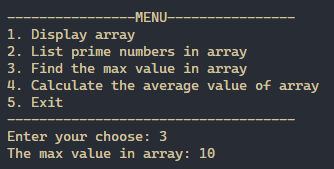
\includegraphics[width=10cm]{images/img5_3.PNG}
	\caption{Chụp màn hình chức năng tìm giá trị lớn nhất với dữ liệu mảng đầu vào như trên.}
\end{figure}

\begin{figure}[H]
	\centering
	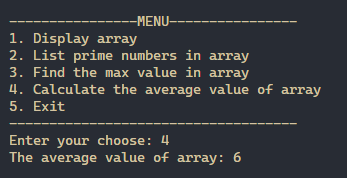
\includegraphics[width=10cm]{images/img5_4.PNG}
	\caption{Chụp màn hình chức năng tính trung bình mảng với dữ liệu mảng đầu vào như trên.}
\end{figure}

\begin{figure}[H]
	\centering
	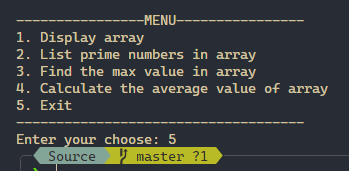
\includegraphics[width=10cm]{images/img5_5.PNG}
	\caption{Thoát chương trình.}
\end{figure}

\begin{figure}[H]
	\centering
	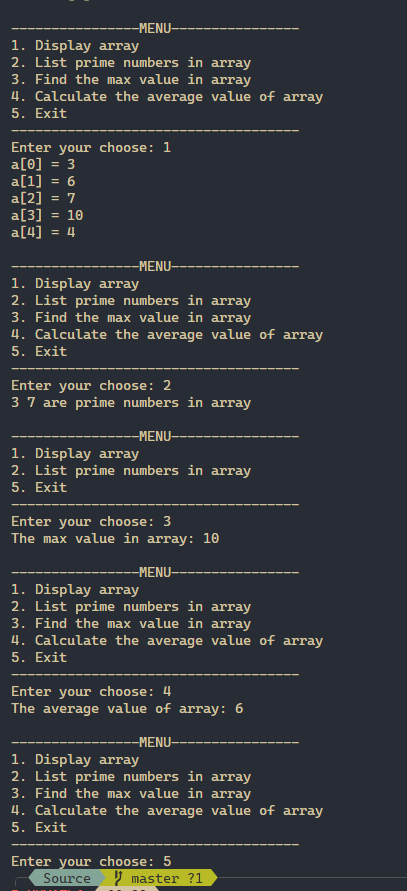
\includegraphics[width=10cm]{images/img5_6.PNG}
	\caption{Menu sẽ tiếp tục lặp lại cho đến khi chọn thoát.}

\end{figure}
